
%\usepackage{graphics} is needed for \includegraphics
\begin{figure}[htp]
\begin{center}
 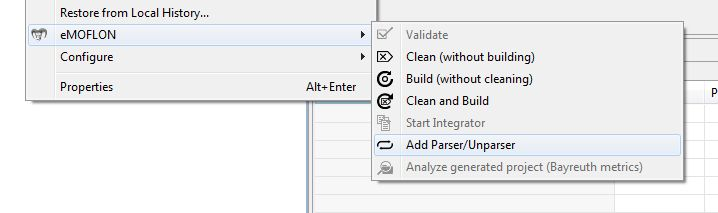
\includegraphics[width=0.8\textwidth]{pics/moca/2TextToMocaTree/1-AddParserAndUnparserWizard}
  \caption{Invoking the \texttt{Add Parser/Unparser} wizard} 
  \label{moca-1-AddParserAndUnparserWizard}
\end{center}
\end{figure}

\begin{enumerate}
\item[$\blacktriangleright$] Right-click on the project
\texttt{DictionaryCodeAdapter} $>$ eMOFLON $>$ Add Parser/Unparser (Fig
\ref{moca-1-AddParserAndUnparserWizard})
\end{enumerate}

%\usepackage{graphics} is needed for \includegraphics
\begin{figure}[htp]
\begin{center}
 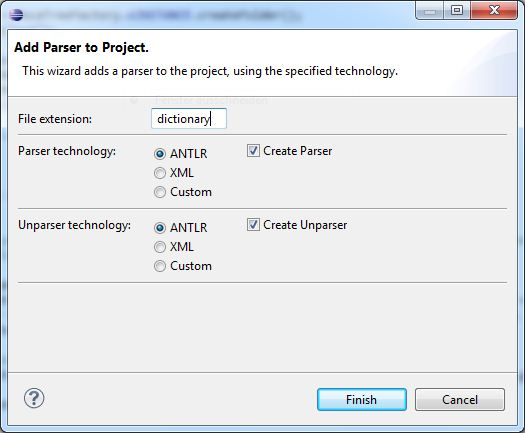
\includegraphics[width=0.7\textwidth]{pics/moca/2TextToMocaTree/2-AddParser}
  \caption{Add Parser/Unparser}
  \label{moca-2-AddParser}
\end{center}
\end{figure}
 
\begin{enumerate}
\item[$\blacktriangleright$] Enter ``dictionary'' as file extension. (Fig
\ref{moca-2-AddParser})
\end{enumerate}
 
%\usepackage{graphics} is needed for \includegraphics
\begin{figure}[htp]
\begin{center}
 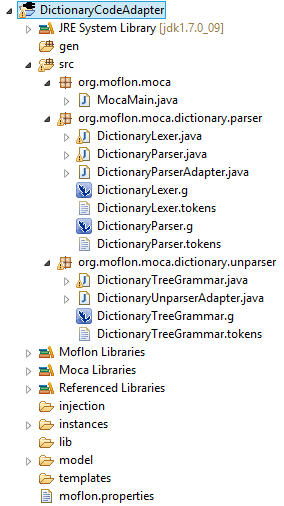
\includegraphics[width=0.6\textwidth]{pics/moca/2TextToMocaTree/3-WizardResult}
  \caption{Workspace after wizard finishes}
  \label{moca-3-WizardResult}
\end{center}
\end{figure}

\begin{enumerate}
\item[$\blacktriangleright$] Add lexer and parser grammars 
\end{enumerate}
 
%\usepackage{graphics} is needed for \includegraphics
\begin{figure}[htp]
\begin{center}
 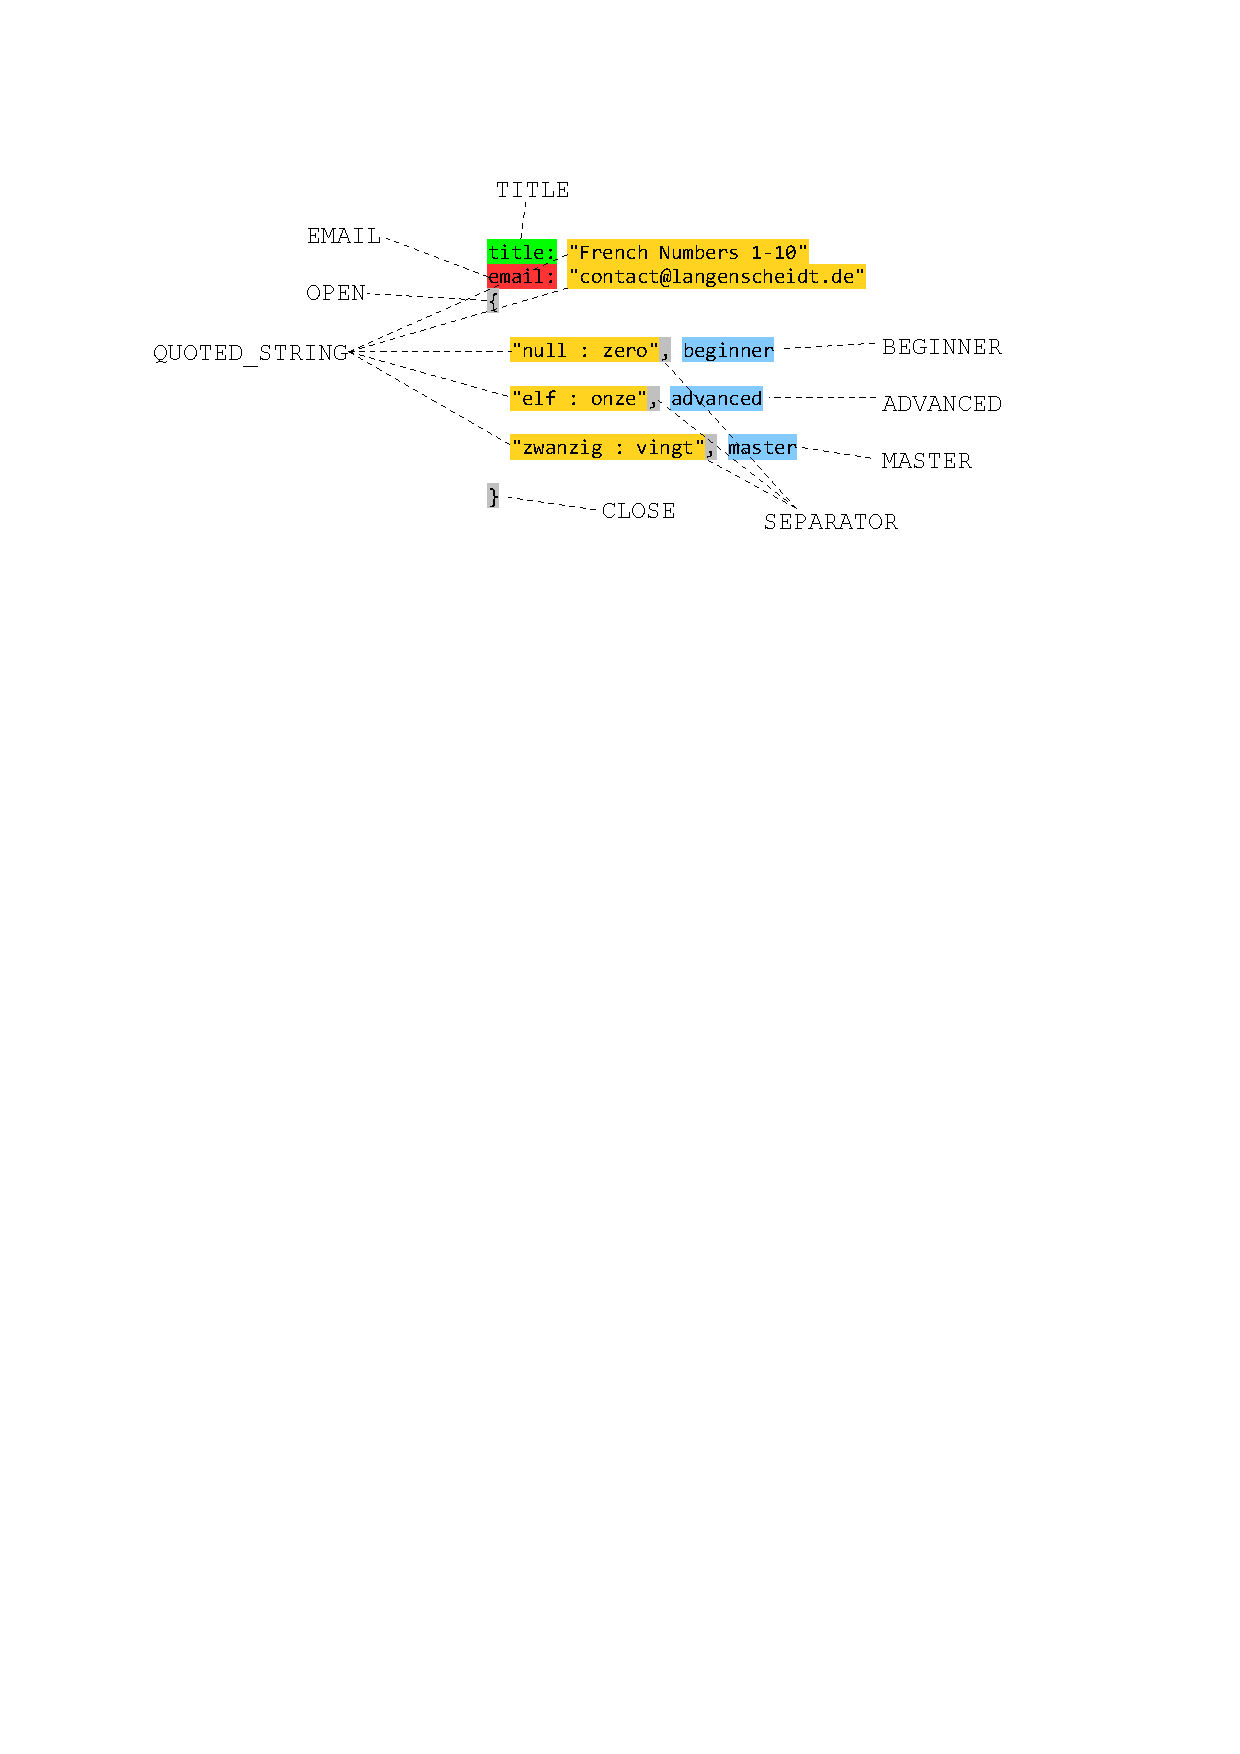
\includegraphics[width=\textwidth]{pics/moca/2TextToMocaTree/4-tokens}
  \caption{Tokens of the Dictionary DSL}
  \label{moca-4-Tokens}
\end{center}
\end{figure}
   
%\usepackage{graphics} is needed for \includegraphics
\begin{figure}[htp]
\begin{center}
 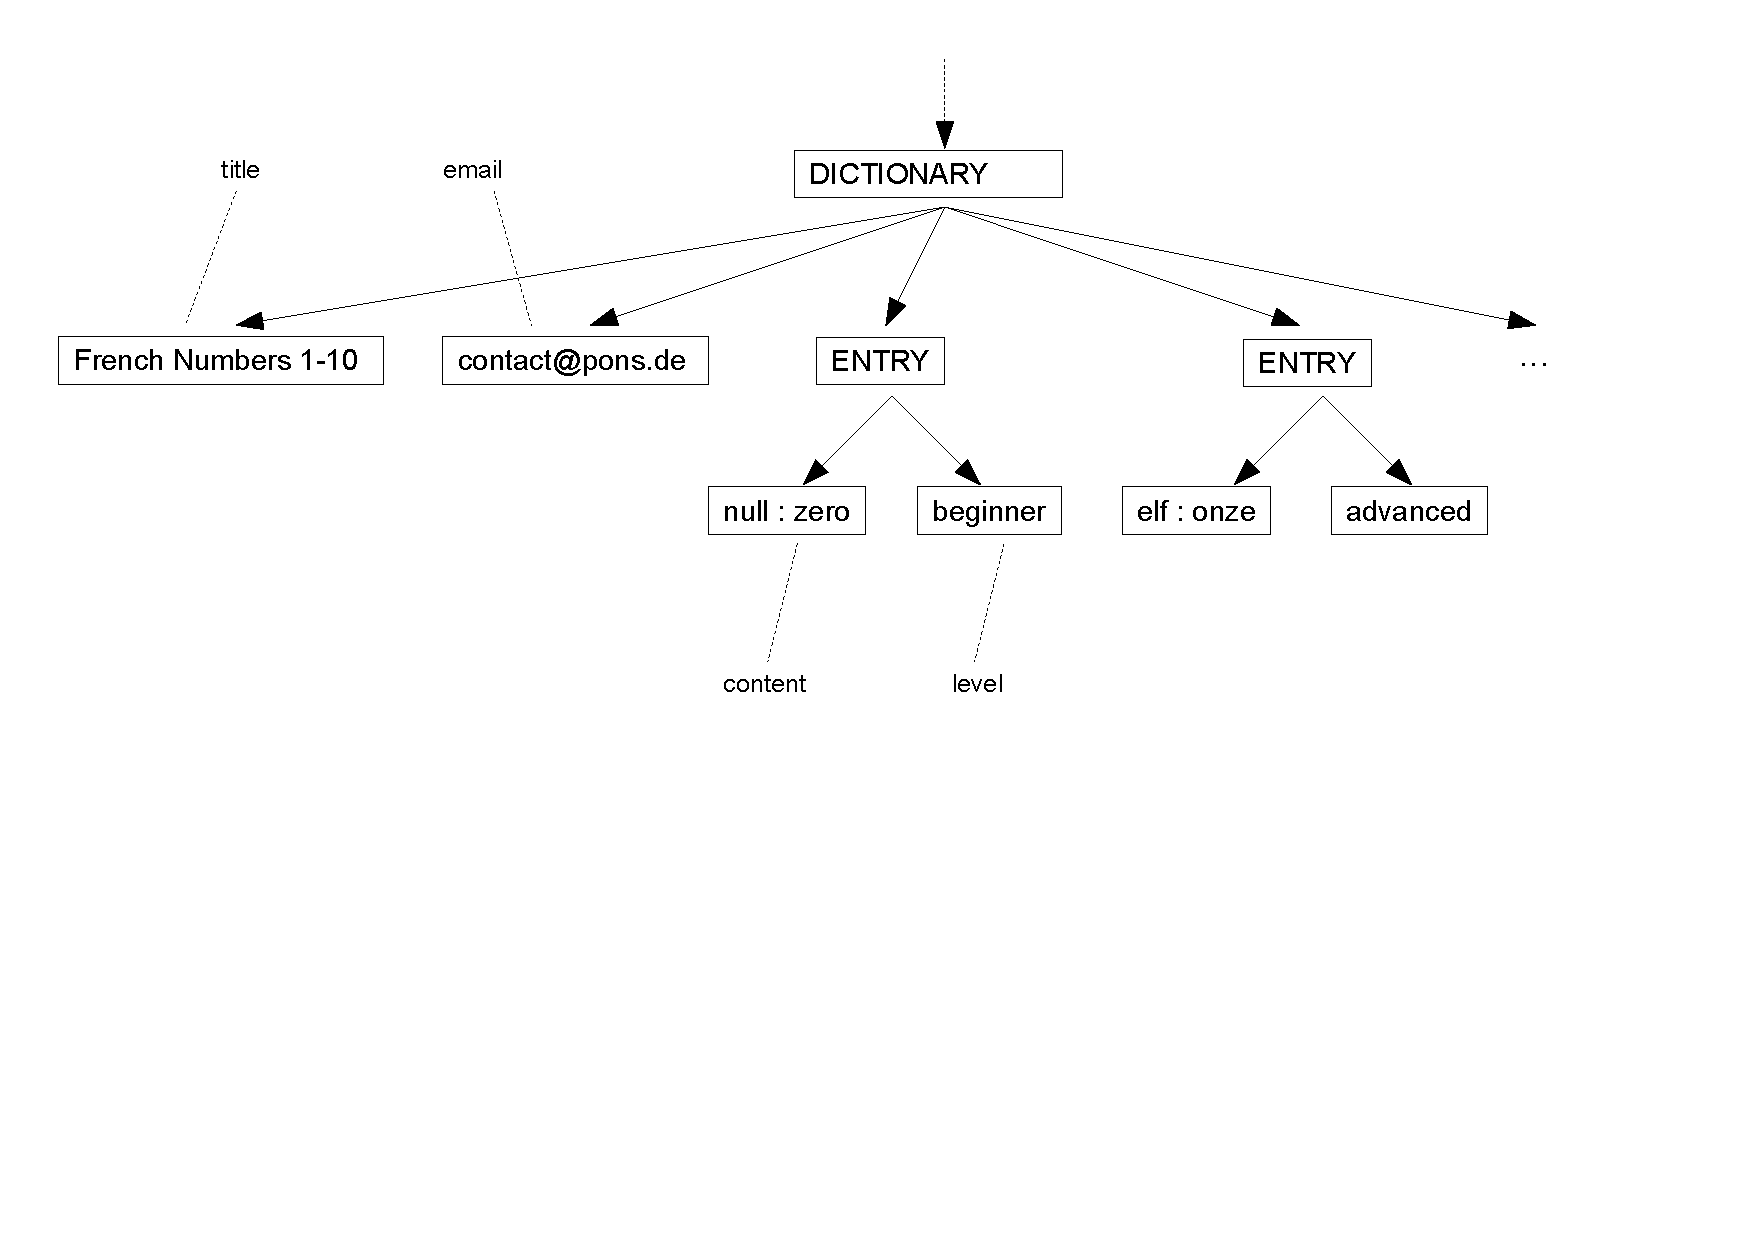
\includegraphics[width=\textwidth]{pics/moca/2TextToMocaTree/5-tree}
  \caption{MocaTree structure}
  \label{moca-5-Tree}
\end{center}
\end{figure}

%\usepackage{graphics} is needed for \includegraphics
\begin{figure}[htp]
\begin{center}
 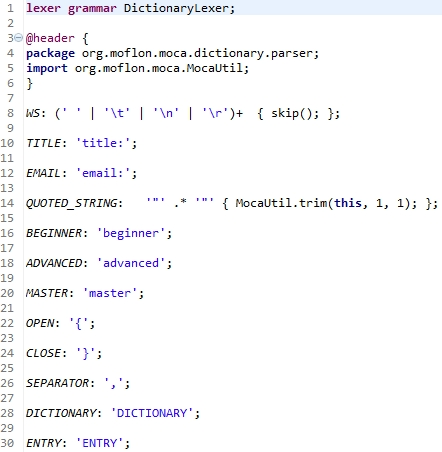
\includegraphics[width=0.7\textwidth]{pics/moca/2TextToMocaTree/6-lexer}
  \caption{Lexer grammar}
  \label{moca-6-lexer}
\end{center}
\end{figure}

%\usepackage{graphics} is needed for \includegraphics
\begin{figure}[htp]
\begin{center}
 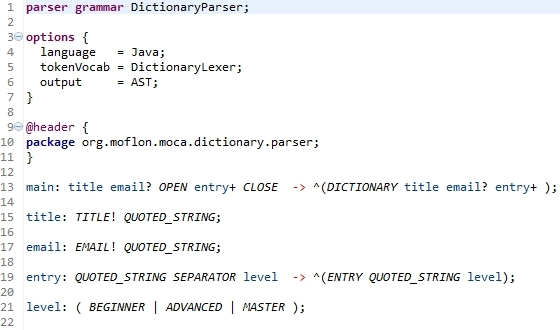
\includegraphics[width=0.9\textwidth]{pics/moca/2TextToMocaTree/7-parser}
  \caption{Parser grammar}
  \label{moca-7-parser}
\end{center}
\end{figure}

\begin{enumerate}
\item[$\blacktriangleright$] Run MocaMain
\end{enumerate}

%\usepackage{graphics} is needed for \includegraphics
\begin{figure}[htp]
\begin{center}
 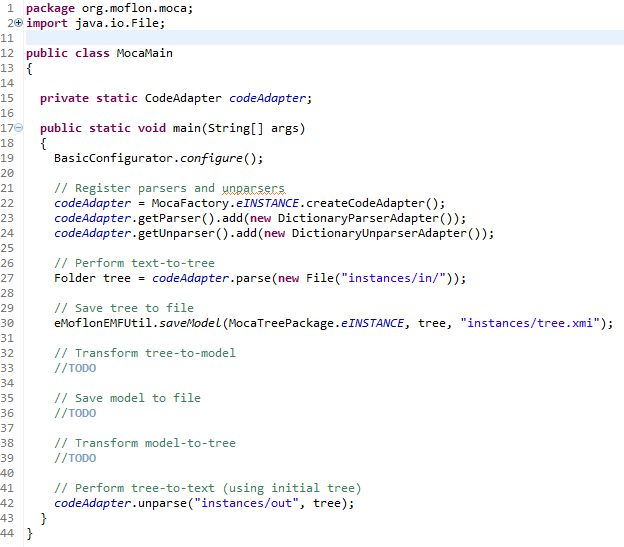
\includegraphics[width=0.8\textwidth]{pics/moca/2TextToMocaTree/8-MocaMain}
  \caption{Generated main method}
  \label{moca-8-MocaMain}
\end{center}
\end{figure}

%\usepackage{graphics} is needed for \includegraphics
\begin{figure}[htp]
\begin{center}
 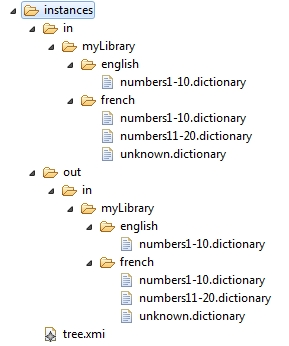
\includegraphics[width=0.5\textwidth]{pics/moca/2TextToMocaTree/9-ParseResult1}
  \caption{Directory \texttt{instances} after parsing}
  \label{moca-9-ParseResult1}
\end{center}
\end{figure}
 

%\usepackage{graphics} is needed for \includegraphics
\begin{figure}[htp]
\begin{center}
 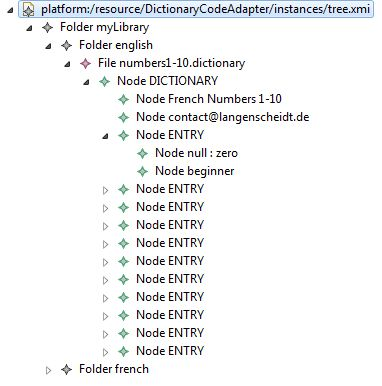
\includegraphics[width=0.5\textwidth]{pics/moca/2TextToMocaTree/10-ParseResult2}
  \caption{MocaTree created by Parser}
  \label{moca-10-ParseResult2}
\end{center}
\end{figure}


